\documentclass[SE,authoryear,lsstdraft,toc]{lsstdoc}
\input{meta}

% Package imports go here.

\usepackage{graphicx}
\usepackage{caption}
\usepackage{subcaption}

% Local commands go here.
\newcommand{\mcat}{m_{\mathrm{cat}}}
\newcommand{\mtrue}{m_{\mathrm{true}}}
\newcommand{\deltam}{\delta_m}
\newcommand{\Deltam}{\Delta\,m}
\newcommand{\etron}{e^{-}}
\newcommand{\mobs}{m_b^{\mathrm{obs}}}
\newcommand{\mstd}{m_b^{\mathrm{std}}}
\newcommand{\Sobs}{S_b^{\mathrm{obs}}}
\newcommand{\Sstd}{S_b^{\mathrm{std}}}
\newcommand{\Iobs}{\mathcal{I}_0^{\mathrm{obs}}}
\newcommand{\Istd}{\mathcal{I}_0^{\mathrm{std}}}

%If you want glossaries
%\input{aglossary.tex}
%\makeglossaries

\title{Rubin Baseline Calibration Plan}

% Optional subtitle
% \setDocSubtitle{A subtitle}

\author{%
Parker Fagrelius, Eli Rykoff
}

\setDocRef{SITCOMTN-086}
\setDocUpstreamLocation{\url{https://github.com/lsst-sitcom/sitcomtn-086}}

\date{\vcsDate}

% Optional: name of the document's curator
% \setDocCurator{The Curator of this Document}

 \setDocAbstract{
 Current baseline plan for the year 1 minimum viable product as delivered for ORR.
 }

% Change history defined here.
% Order: oldest first.
% Fields: VERSION, DATE, DESCRIPTION, OWNER NAME.
% See LPM-51 for version number policy.
 \setDocChangeRecord{
   \addtohist{1}{2023-XX-XX}{Unreleased.}{Parker Fagrelius}
 }

\setcounter{tocdepth}{2}

\begin{document}

% Create the title page.
\maketitle
% Frequently for a technote we do not want a title page  uncomment this to remove the title page and changelog.
% use \mkshorttitle to remove the extra pages


\section{Introduction}

The basic question of photometric calibration of an astronomical survey is how
to take raw counts output from the camera (in arbitrary Analog-Digital Units
(ADU)) and convert these to calibrated fluxes in nanoJansky (nJy).  In order
for this procedure to yield uniform results across the camera and the sky, it
must take into account variations that are both achromatic (``gray'') and
chromatic, that latter of which depend on the spectral energy distribution (SED) of each
object.  This includes variations in the atmosphere as a function of time and
airmass; spatial variations in the filter and detectors; pixel size variations;
and various sensor effects such as charge transfer ineffeciency (CTI) and the
Brighter Fatter Effect (BFE).

This technote describes the baseline photometric calibration plan for Rubin
Commissioning and the first year of data release production for the LSST
Survey.  This includes plans on performing instrumental signature reduction
(ISR), which is also known as ``detrending''; correct flat-fielding;
background/foreground subtraction; and derivation of a uniform photometric
calibration over the full survey.  It also includes plans for generating
``calibration frames'' such as bias, darks, and various types of flats,
incorporating LEDs, a class 4 tunable laser, and a novel Collimated Beam
Projector (CBP).  We expect that this is not the final calibration plan for the
LSST survey, but rather a first minimal viable product suitable for the first
year of survey observations to meet our required goals for repeatability and
uniformity.  Further improvements are planned to incorporate more effects,
although our plan is to take as much calibration data early on to be able to
reprocess early data with improved algorithms.

The calibration plan in this technote is heavily influenced by the Dark Energy
Survey, which achieved better than $2~\mathrm{mmag}$ uniformity over
$5000\,\mathrm{deg}^2$ in the Southern sky~(Rykoff et al. 2023).  In
particular, we refer the reader to Bernstein et al. 2017 (henceforth B17) and
Burke, Rykoff, et al. 2018 (henceforth BR18).

\section{Requirements}
The requirements on calibration are defined in the Science Requirements Document (LPM-17). The photometric quality and accuracy of the LSST data products is driven by four main components:
\begin{enumerate}
    \item Relative photometry (repeatability)
    \item Stability across the sky (spatial uniformity)
    \item Relative accuracy (color zero-points)
    \item Transfer to physical flux scale (external absolute photometry)
\end{enumerate}

The requirements for photometric calibration accuracy are specified using the
following error decomposition (valid in the limit of small errors):
%
\begin{equation}
    \mcat = mtrue +\sigma+\deltam (x,y,\theta,\alpha,\delta,\mathrm{SED},t)+\Deltam
\end{equation}
%
where $\mtrue$ is the true magnitude defined by eqs. 4 and 7, $\mcat$ is the
cataloged LSST magnitude, $\sigma$ is the random photometric error (including
random calibration errors and count extraction errors), and $\Deltam$ is the
overall (constant) offset of the internal survey system from a perfect AB
system (the six values of $\Deltam$ are equal for all the cataloged objects).

Here, $\deltam$ describes the various systematic dependencies of the internal
zeropoint error around $\Deltam$, such as position in the field of view $(x,
y)$, the normalized system response ($\theta$), position on the sky
($\alpha$,$\delta$), and the source spectral energy distribution(SED).  Note
that the average of $\deltam$ over the cataloged area is 0 by construction.

The SRD allocates error specifications for the griz bands, with a 50\% increase
expected for $u$ and $y$ bands. These high level allocations are further broken
down to three main elements in Observatory System Specifications
(LSE-30). These are Instrument Throughput, Atmospheric Transmittance, and
Reference Star Catalogs. The full functional error budget can be found in LSST
Document-9553.

\begin{table}
\centering
\begin{tabular}{|c|c|c|c|c|}
\hline
Design Spec & Repeatability & Uniformity & Color Accuracy & External Absolute  \\
 (millimag) &  &  &  & Photometry \\
\hline\hline
Overall Specification & 5 &  10 & 5 & 10 \\
Instrument Throughput & 3 & 2 & 3 & -  \\
Atmospheric Transmittance & 3.5 & 4 & 3 & - \\
Reference Catalog & 2.5 & 9 & 3 & - \\
\hline
\end{tabular}
\caption{TABLE NAME NEEDED}
\label{tab:table1}
\end{table}
%
where $\textrm{m}_{true}$ is the true magnitude defined by eqs. 4 and 7,
$\textrm{m}_{cat}$ is the cataloged LSST magnitude, $\sigma$ is the random
photometric error (including random calibration errors and count extraction
errors), and $\Deltam$ is the overall (constant) offset of the internal survey
system from a perfect AB system (the six values of $\Deltam$ are equal for all
the cataloged objects).  Here, $\deltam$ describes the various systematic
dependencies of the internal zeropoint error around $\Deltam$, such as position
in the field of view (x, y), the normalized system response ($\theta$),
position on the sky ($\alpha$, $\delta$), and the source spectral energy
distribution (SED).  Note that the average of $\deltam$ over the cataloged area
is 0 by construction.

The SRD allocates error specifications for the griz bands, with a 50\% increase
expected for $u$ and $y$ bands.  These high level allocations are further broken
down to three main elements in Observatory System Specifications (LSE-30).
These are Instrument Throughput, Atmospheric Transmittance, and Reference Star
Catalogs.  The full functional error budget can be found in LSST Document-9553.

\begin{table}
    \begin{tabular}{|c|c|c|c|c|}
        \hline
        Design Spec (millimag) & Repeatability & Uniformity & Color Accuracy & Abs. Photometry \\
        \hline
        \hline
        Overall Specification & 5 & 10 & 5 & 10 \\
        \hline
        Instrument Throughput & 3 & 2 & 3 & - \\
        \hline
        Atmospheric Transmittance & 3.5 & 4 & 3 & - \\
        \hline
        Reference Catalog & 2.5 & 9 & 3 & - \\
        \hline
    \end{tabular}

\end{table}

From these functional requirements, requirements are allocated to the Telescope
\& Site (LSE-60) and Data Management (LSE-61) systems to ensure that the
functional requirements are met.

\section{Instrumental Signature Reduction (ISR)}

In this section, we describe the instrument signature removal (ISR) for
LSSTCam.  After the photons hit the detector surface, there are a number of
sensor effects that alter the image as photoelectrons are produced, collected
in the detector, clocked and read out, and sent through the amplifier(s) to the
analog-to-digital converter (ADC).  Each of these steps can imprint an effect,
including adding noise, non-linearities, cross-talk, etc.  Our goal in ISR is
to apply corrections ``in reverse'' to go from the raw camera output of Analog
to Digital Units (ADU) in 16 amplifiers to a ``post ISR'' image in units of
electrons ($\etron$) that are equiavlent to the number of photocarriers
produced in each pixel incident on the camera.  In this stage we do not correct
for quantum efficiency as a function of wavelength, as that requires knowledge
of each individual source SED.  We leave the wavelength dependent effects to
the photometric calibration described in Section~\ref{sec:photocal}.

% If necessary we can add in a section about differential non-linearity corrections.

\subsection{Overscan Correction}

The first operation we must perform is ``overscan correction'' to remove the
amplifier bias level.  Unfortunately, for many channels the bias level in
LSSTCam is not completely stable with time, and thus we support a somewhat
complicated overscan subtraction routine, using both serial overscan (the
additional readout at the end of each row) and parallel overscan (the
additional readout at the end of each column).  The software may be configured
to use specialized overscan settings on a per-detector and per-amplifier basis.

In our default mode, we first perform row-by-row serial overscan correction to
remove the bias level as well as possible bias drift and jumps.  We have X
overscan pixels per row, and we take the median of each row, skipping the first
two columns, using the LSST Science Pipelines integer median sampling algorithm
(ref?).  This introduces approximately XX ADU of noise, which may or may not be
comparable to our read noise (TBD).

For some amplifier channels we need to additionally perform parallel overscan
subtraction.  One challenge of the parallel overscan subtraction is that hot
columns and saturated stars bleed into the parallel overscan region, making
these columns unusable for parallel overscan subtraction.  In addition, these
bright signals inject a crosstalk signal into the other crosstalk regions.
Therefore, prior to parallel overscan subtraction we perform crosstalk
correction on just the parallel overscan region (see Section~\ref{sec:xtalk}
for details on the crosstalk correction algorithm).  Additionally, we mask the
regions with saturated parallel overscan and interpolate along the columns.
Finally, we perform column-by-column parallel overscan correction.

\subsection{Saturation Flagging}

After overscan correction, we must flag pixels that are deemed to be
``saturated'' to ensure that these are handled correctly in the following ISR
steps.  We have yet to determine which definition of saturation/full-well is
appropriate.  Possible definitions include (a) the PTC turnoff (where the
variance of pixel estimates deviates significantly from Poisson); (b) the level
at which the charge-transfer-inefficiency (see Sec~\ref{sec:cti}) cannot be
corrected; (c) the maximum possible observed value in a pixel; (d) the level above
which the E2V sensors exhibit persistence effects.

\subsection{Linearity Correction}

The response of the readout system is not completely linear, as the
amplification of the voltage in the sense node of the amplifier may not be
completely linear.  [There are other sources of non-linearity; this seems to be
the best place to do this correction, and I would like RHL help in describing
these.]

Our linearity correction model is a multi-node spline as original defined by
P. Astier (ref?).  The linearity correction per amplifier is derived from a
series of flat pairs illuminated at different flux levels and contemporaneously
monitored with a photodiode.  We need to take special care in accounting for
the different illumination patterns when the LED is used with different current
levels, as well as stray light, and gain variation as a function of temperature
(described below).

\subsection{Crosstalk Correction}

Every time a pixel is clocked out through an amplifier, there is an effect on
the voltages in the other amplifiers on the same detector.  This crosstalk
signal must be corrected by a full matrix for each detector that describes the
effect of each ``source'' amplifier on every ``target'' amplifier.  The
crosstalk values for LSSTCam are around XX.  Furthermore, there is a
non-linearity in the crosstalk response of the LSSTCam amplifiers.  These are
modeled as a first-order correction to the crosstalk matrix as a function of
source signal level (A. Snyder, thesis).

The crosstalk matrix coefficients were derived by A. Snyder using ``blobs''
projected onto LSSTCam.  I do not know how much detail is needed here.

\subsection{Bias Subtraction}

After correcting for all of these effects, there may be some residual imprint
of some bias structure.  To generate a bias frame to subtract from the image we
take a series of zero-second integrations, perform the above ISR correction
steps in order, and take the median.  Note that it is important to perform
crosstalk correction prior to bias frame creation to ensure that the crosstalk
signal from hot columns is corrected or else these will get imprinted on all of
the amplifier segments which is undesirable.

\subsection{Gain Normalization}

In this step we convert the units of each amplifier from ADU to $\etron$ using
the gain measurement.  This is a two step process, as we know that the gain has
a small dependence on readout board (REB) temperature ($\approx
0.06\%/{^\circ}C$), and we must correct for any small temperature shifts to
ensure that ...

Using the photon transfer curve (PTC) analysis (ref) we are able to measure the
gain ($\etron/\mathrm{ADU}$) for each amplifier

\subsection{CTI Correction}

\subsection{Variance Plane Creation}

\subsection{Defect Masking and Interpolation}

\subsection{Dark Subtraction}

\subsection{Brighter-Fatter Correction}

\subsection{Applying Flat Fields}

\section{Photometry with Chromatic Corrections}
\label{sec:photocal}

The fundamental goal of photometric calibration is to estimate the surface
brightness of sources across the full sky in a uniform way, as would be
measured at the top of the atmosphere (TOA).  Our general outline for uniform
photometry follows DES and specifically B17 and BR18.  Our ground-based
telescope will count only a fraction of photons from a celestial source that
reaches the top of the Earth's atmosphere after attenuation from the
atmosphere, filters, optics, and detector quantum efficiency.

Our overall photometry plan follows BR18, in particular the use of the Forward
Global Calibration Method (FGCM).  This global calibration algorithm uses
repeated observations of stars in multiple bands, through multiple instrumental
and atmospheric bandpasses, to simultaneously constrain the atmospheric model
as well as standardized TOA star fluxes over a wide range of star colors.

\subsection{Chromatic Corrections}

For broadband observations through the ${u,g,r,i,z,y}$ filters, the number of
photoelectrons ($\etron$) produced by a source in a pixel is proportional to the
integral of the TOA flux $F_\nu(\lambda)$ (the source spectral energy
distribution, or SED) weighted by the observation
transmission function, $S_b(x, y, \mathrm{alt}, \mathrm{az}, t, \lambda)$ in a
given filter $b$.  We discuss the effect of integrating over the point spread
function (PSF) and pixel size variations below.
%
\begin{equation}
\etron_b = A \int_0^{\Delta T}dt \int_0^\infty
F_\nu(\lambda) S_b(x, y, \mathrm{alt}, \mathrm{az}, t, \lambda)
\frac{d\lambda}{h_{\mathrm{Pl}}\lambda},
\end{equation}
%
where $A$ is the area of the telescope pupil and $\Delta\,T$ is the duration of
the exposure.  The position ${x, y}$ is the location in the focal plane;
${\mathrm{alt}, \mathrm{az}}$ are the altitude and azimuth of the observation
(the altitude being the more important driver of the variation of the
transmission by the atmosphere as a function of airmass).  The units of flux
$F_\nu(\lambda)$ are
$\mathrm{erg}\,\mathrm{cm}^{-2}\,\mathrm{s}^{-1}\,\mathrm{Hz}^{-1}$, and the
factor $\frac{d\lambda}{h_{\mathrm{Pl}\lambda}}$ counts the number of photons
per unit energy at a given wavelength, where $h_{\mathrm{Pl}}$ is Planck's
constant.

Following BR18, we definte the ``observed passband'', which is position- and
time-dependent, as such:
%
\begin{equation}
\Sobs \equiv S_b(x, y, \mathrm{alt}, \mathrm{az}, t, \lambda).
\end{equation}

Following Fukugita et al. (1996), we define the AB magnitude of a source to be:
%
\begin{equation}
\mobs = -2.5\,\mathrm{log}_{10} \left ( \frac{\int_0^{\infty}
  F_\nu(\lambda)\,\Sobs\,\lambda^{-1}d\lambda}{\int_0^{\infty}
  F^{\mathrm{AB}}\,\Sobs\,\lambda^{-1}d\lambda} \right ),
\end{equation}
%
where $F^{\mathrm{AB}} = 3631\,\mathrm{Jy}$.  Putting this together with the
above equation and simplifying we get:
%
\begin{equation}
\mobs = -2.5\,\mathrm{log}_{10}(\etron_b) +
2.5\,\mathrm{log}_{10}({\Delta}T) + 2.5\,\mathrm{log}_{10}(\Iobs) +
\mathrm{ZPT}^{\mathrm{AB}},
\end{equation}
%
where

\begin{equation}
\mathrm{ZPT}^{\mathrm{AB}} = 2.5\,\mathrm{log}_{10}
 \left (\frac{A\,F^{\mathrm{AB}}}{h_{\mathrm{Pl}}} \right ),
\end{equation}

and $Iobs$ is defined as the integral over the observed passband $b$:
%
\begin{equation}
\label{eqn:Iobs}
\Iobs(b) \equiv \int_0^\infty \Sobs(\lambda)\,\lambda^{-1}\,d\lambda.
\end{equation}
%

Note that in the formulation so far we are limited by the variety of observed
passbands that are encountered in a survey, due to variations in instrument
over the focal plane and atmosphere over time.  Furthermore, these equations
require knowledge of the wavelength dependence of the source SED.  Therefore,
we define a ``standard'' magnitude as the broadband magnitude that would be
measured if a given source were observed through a standard passband $Sstd$
that we are free to choose:
%
\begin{equation}
\mstd \equiv -2.5\,\mathrm{log}_{10} \left ( \frac{\int_0^\infty
  F_\nu(\lambda)\,\Sstd\,\lambda^{-1}\,d\lambda}{\int_0^\infty
  F^{\mathrm{AB}}\,\Sstd\,\lambda^{-1}\,d\lambda} \right ).
\end{equation}
%
The difference between this standard magnitude and the observed magnitude is
then:
%
\begin{equation}
\label{eqn:deltastd}
\delta_b^{\mathrm{std}} \equiv \mstd - \mobs\\
= 2.5\,\mathrm{log}_{10}(\Istd(b)/\Iobs(b))\\
+ 2.5\,\mathrm{log}_{10} \left ( \frac{\int_0^{\infty}
  F_\nu(\lambda)\,\Sobs(\lambda)\,\lambda^{-1}\,d\lambda}{\int_0^{\infty}
  F_\nu(\lambda)\,\Sstd(\lambda)\,\lambda^{-1}\,d\lambda} \right ),
\end{equation}
%
where $\Istd$ is defined as in Eqn.~\ref{eqn:Iobs}.

The decomposition in Eqn.~\ref{eqn:deltastd} is very useful.  First of all, the
first term is independent of the SED, and the SED-dependent ``chromatic
correction'' is entirely in the second term.  Second, the chromatic correction
term goes to zero if either (a) the source SED is completely flat (as with the
reference AB spectrum or (b) the observed passband $\Sobs(b)$ is equal to the
standard passband $\Sstd(b)$.  Therefore, it is important to choose a standard
passband as close to the ``typical'' observing conditions as possible in order
to minimize the chromatic corrections, and to ensure that averaging over many
observed passbands tends toward the mean (standard) passband.  For LSSTCam this
is made more challenging by the different shapes of the QE curves of the two
types of detectors (E2V and ITL), and so we must decide whether to choose one
or the other shape as the standard, or to ``split the baby'' and choose
something in the middle that is representative of neither.

\subsection{Observed Passbands}

We assume that the instrumental and atmospheric components of the observed
passband are independent, and therefore we can decompose $\Sobs$ as such:
%
\begin{equation}
\Sobs(\lambda) = S_b^{\mathrm{inst}}(x, y, t,
\lambda)\,S^{\mathrm{atm}}(\mathrm{alt}, \mathrm{az}, t, \lambda),
\end{equation}
%
where $S_b^{\mathrm{inst}}$ is the instrumental component that depends on
location in the detector and focal plane, as well as time and wavelength, and
$S_b^{\mathrm{atm}}$ is the atmospheric component that depends on pointing in
the sky.  We address each of the instrumental and atmospheric transmission
curves in turn.

\subsection{Instrumental Response}

We can decompose the instrumental response into different parts that depend on
the focal plane and time in different ways.  Our initial decomposition is:
%
\begin{equation}
S_b^{\mathrm{inst}}(x, y, t, \lambda) = k_b\,S^{\mathrm{refflat}}(x, y,
\lambda)\,S^{\mathrm{optics}}(t, \lambda)\,S^{\mathrm{CBP}}(x, y, \lambda),
\end{equation}
%
where $S^{\mathrm{refflat}}$ is the ``reference flux flat'' that normalizes the
system response to focused light; $S^{\mathrm{optics}}$ describes the change in
the opacity of the optical system over time; $S^{\mathrm{CBP}}$ is the
in-situ chromatic throughput of the system as measured by the collimated beam
projector; and $k_b$ is an overall throughput constant at the start of the
survey that can be determined with observations of standard stars/white dwarfs.

\subsubsection{Change in Opacity of Optical System}

We break out the $S^{\mathrm{optics}}(t, \lambda)$ as a separate component,
because to first order the dust on the optics and mirror build up smoothly over
time, more frequently than we can or want to determine ``absolute'' calibrated
throughput measurements.  In the original DES formalism described in BR18 this
was only a gray term without wavelength dependence, with offsets determined
whenever there was a mirror wash or hardware change.  Further experience with
DES and Hyper Suprime Cam Special Survey Program (HSC; need ref) demonstrated
that the mirror coating degrades chromatically over time due to molecular
changes.  This chromatic change is visible in all bands, but is most dramatic
in the bluest bands.  Therefore, we must allow a smooth degradation of
$S^{\mathrm{optics}}$ as a function of wavelength (estimated as a first-order
correction; I have to put the math somewhere in here).

\subsubsection{In-situ Measurements of Chromatic Throughput from CBP}

The term $S^{\mathrm{CBP}}$ describes the in-situ chromatic estimate (with an
arbitrary normalization) from the ``static'' CBP: including the filter (as a
function of wavelength and position); the mirrors M1, M2, and M3 (as a function
of wavelength); the lenses L1, L2, ?? (as a function of wavelength); and the
detector quantum efficience (QE) as a function of position.  For Y1
calibrations we assume that $S^{\mathrm{CBP}}(x, y, \lambda)$ is constant for each
detector, and will refine this in future versions of the calibration system.
Overall, we expect that the CBP measurements should agree with lab data for
detector QE and vendor measurements of filter throughput as a function of
position.  Note that we could use monochromatic flats like the DECal system
(ref) to achieve the same in-situ chromatic throughput estimation, although
ghosting due to unfocused light makes this much easier with the CBP.

\subsubsection{Reference Flux Flats}

The term $S^{\mathrm{refflux}}$ is the reference flux flat which normalizes the
response to focused light~(see, e.g. B17).  Nominally, this has chromatic
variations at small scales (particularly the ITL detectors in the bluest
bands), but for Y1 we are assuming any chromatic variations are assumed to be
constant at the detector scale and described by the
$S^{\mathrm{CBP}}(\lambda)$.  Therefore, this term is just the achromatic
(gray) portion of the instrumental throughput which can vary from pixel to
pixel.

The reference flux flat has a few key differences from the ``dome flat'' which
is obtained by measuring the response to a Lambertian source of light such as
the dome screen.  First of all, the dome flat contains a factor of the pixel
area $\Omega(x, y)$, which means that it assumes pixel size variations are QE
variations.  Second, there are differences in focused and scattered light
patterns from a flat field screen and distant sky sources.  Third, the dome
flat is contaminated by scattered light.  Finally, the SED of the dome flat
does not match the reference spectrum.  This final problem we will fix in
future data processing by synthesizing broadband flats from narrow-band flats.
Nevertheless, we still start with dome flats as they are the most efficient way
of measuring the relative response of all the billions of pixels in LSSTCam on
small scales.

The dome flat is a good start for estimating the reference flax flat, but has
issues at small scales and large scales.  At small scales, there are lateral
electric field effects such as ``tree rings'' and the ``picture frame'' that
are pixel size variations that show up as apparent QE variations in the dome
flat.  At large scales, the response to focused light is different than the
dome flat which includes unfocused and scattered light.

To handle lateral electric field effects we fit templates based on our physical
knowledge of the detectors.  This includes radial templates for tree rings with
a fixed center, and square templates around the edge of the detectors.  The
exact methodology is TBD.

To handle large scale variations for LSST Y1 we use a ``star flat'' generated
from a sequence of multi-band dithered observations of a moderately dense star
field.  These observations are cross-calibrated using FGCM to generate
per-detector polynomial approximations of the throughput relative to the dome
flat at scales of hundreds of pixels and greater.  By making use of stars of
various colors, the FGCM solution can approximate the star flat terms for a
flat reference spectrum.

In the future, we plan to use what we call the ``dynamic'' CBP, where the
synthetic stars from the CBP are dithered around the full focal plane.  The
advantage of this is that the response can be more carefully controlled, and it
can be performed in narrow wavelength steps to build up the dynamic CBP star
flat with any arbitrary spectrum.  The software to perform this analysis will
not be ready by the completion of construction.

\subsection{Atmosphere Response}

The attenuation of light due as it propagates through the atmosphere includes
absorption and Rayleigh scattering from molecular constituents (primarily $O_2$
and $O_3$); absorption by preciptable water vapor (PWV), Mie scattering by
airborne particulate aerosols that have physical sizes comparable to the
wavelength of visible light; and shadowing by ice crystals and water droplets
in clouds that is independent of wavelength.

This can be summarized with the following equation:
%
\begin{equation}
S^{\mathrm{atm}}(\mathrm{alt}, \mathrm{az}, t, \lambda) =
S^{\mathrm{molecular}}(\mathrm{bp}, \mathrm{zd}, t,
\lambda)\,S^{\mathrm{PWV}}(\mathrm{zd}, t,
\lambda)\,e^{-(X(\mathrm{zd})\,\tau(t, \lambda))},
\end{equation}
%
where $S^{\mathrm{molecular}}$ is the absorption and scattering from dry gasses
(primarily in the u, g, and r bands); $S^{\mathrm{PWV}}$ is the absorption by
water vapor (primarily in the z and y bands); $\tau$ is the aerosol optical
depth (AOD); $X$ is the airmass; and $\mathrm{bp}$ is the barometric pressure.

Following FGCM, we obtain the molecular scattering using MODTRAN (ref) combined
with the barometric pressure, which is obtained as part of the standard suite
of weather data at Cerro Pachon.  Ozone absorption can be parameterized by one
parameter per night.  All constituent throughputs are computed as a function of
zenith distance (airmass) in finite steps and interpolated at each wavelength step.

The PWV may vary through the night and as a function of position in the sky.
In the FGCM default model the PWV is allowed to vary via a smooth quadratic
function through the night.  It may also be estimated per visit in the z and y
bands by using the relative shift of stars of different colors.  As above, we
use MODTRAN to determine the absorption as a function of wavelength for a grid
of PWV and zenith distance values which are then interpolated.

The aerosol model is a simple Angstrom model with one particular species:
%
\begin{equation}
\tau(\lambda) = \tau_{7750}\,(\lambda/7750\,\Angstrom)^{-\alpha},
\end{equation}
%
where the normalization $\tau_{7750}$ and optical index $\alpha$ depnd on the
density, size, and shape of the particulates.  As with PWV, the AOD
normalization is allowed to vary linearly through the night, while the optical
index is given a single night.

\subsection{Auxiliary Telescope}

The Auxiliary Telescope (AuxTel) will be in operation during the LSST survey,
obtaining contemporaneous estimates of the atmospheric throughput via low
resolution spectroscopy of bright (sixth magnitude) stars.  The mode of
operation of AuxTel has not yet been finally determined.  We are likely to use
different modes in observing when LSST is targeting $ugri$ bands (where more
care needs to be taken with the aerosols and ozone) and when LSST is targeting
the $zy$ bands (where we need to know the PWV to high precision).

In the first iteration, we plan on using the AuxTel model outputs to validate
the FGCM atmospheric model which is determined from the broadband multi-color
photometry of the stars observed on a given night.  In the future, we may use
AuxTel to provide priors on the atmospheric model fit.  Considerable care will
have to be taken to ensure that outliers from the spectroscopic fits do not
contaminate the model used in the broadband photometry.  We do not plan to use
satellite measurements of atmospheric constituents as priors as the resolution
is low enough to be contaminated by observations of neighboring valleys rather
than the mountain peak where the telescope is sited.

\subsection{Integrating Over Sources}

This short section will discuss PSF modeling and aperture photometry and the
finit size of stars (and galaxies) and the care that needs to be taken with
fluence or surface density images, following B17.


\subsection{Foregrounds and Backgrounds}

What to do about foregrounds and backgrounds, including fringes?  These needs
to be written.

\subsection{ISR Operation}

*TO BE UPDATED AND MOVED*

In this section, we describe the instrument signature removal (ISR) for
LSSTCam.  After the photons hit the detector, there are a number of sensor
effects that alter the image as photoelectrons are produced, they are collected
in the detector, clocked and read out, and sent through the amplifier to the
analog-to-digital converter (ADC).  Each of these steps can imprint an effect,
including noise, non-linearities, cross-talk, etc.  Our goal in ISR is to apply
corrections ``in reverse'' to go from the raw camera output (ADU in 16
amplifiers) to a ``post ISR'' image in units of electrons that are equivalent
to the number of photocarriers produced in each pixel incident on the camera.
In this stage we do not correct for quantum efficiency as a function of
wavelength, as that requires knowledge of each individual source SED.

% If necessary we can add in a section about differential non-linearity corrections.

\subsubsection{Overscan Correction}

The first operation we must perform is ``overscan correction'' to remove the
amplifier bias level.  Unfortunately, the bias level in LSSTCam is not
completely stable with time, and thus we require a somewhat complicated
overscan subtraction routine, using both serial overscan (the additional
readout at the end of each row) and parallel overscan (the additional readout
at the end of each column).

First, we perform row-by-row serial overscan correction to remove possible bias
drift and jumps.  [We are investigating a more complex algorithm for some amplifiers
to reduce row-by-row noise.]  We have X overscan pixels per row, and we take
the median of each row, skipping the first two columns, using the afw integer
median sampling algorithm.  [This needs to be written down or referenced
  somewhere].  This introduces approximately XX ADU of noise, which may or may
not be comparable to our read noise, to be calculated.

Next we need to apply parallel overscan subtraction.  One challenge of the
parallel overscan subtraction is that hot columns and saturated stars bleed
into the parallel overscan region, making these columns unusable for
parallel overscan subtraction.  In addition, these bright signals inject a
crosstalk signal into the other crosstalk regions.  Therefore, prior to
parallel overscan subtraction we perform crosstalk correction on just the
parallel overscan region.  As this is done after serial overscan subtraction
(even into the parallel overscan region) this crosstalk correction does not
require extra source detection or background estimation, as in the standard
crosstalk correction described below.  Additionally, we mask the regions with
the saturated parallel overscan and interpolate these.  Finally, we perform
column-by-column parallel overscan correction.  This should be improved.

Not every amplifier on every detector requires the parallel overscan
correction.  Hopefully by the time we get to commissioning we can specify which
amplifiers are problematic, and add a figure here which shows how that works.
Alternatively, new smoother parallel overscan will help a lot everywhere.

\subsubsection{Bias Subtraction}

Next we subtract off any residual common-mode bias structure by subtracting off
a median ``bias'' frame.  The combination of these is described in Section XX.

\subsubsection{CTI Correction}

We must now correct for charge-transfer inefficiency (CTI).  This is due to the
fact that as charge is clocked along the either the serial direction (sCTI) or
parallel direction (pCTI) some small fraction of charge is left behind.  Full
details of our correction algorithm are in [Broughton et al.?].

\subsubsection{Linearity Correction}

We want to ensure that the response of the number of ADU counts that we measure
is completely linear with the incident photons, over a very wide dynamic
range.  We correct for non-linearities using a 10 node spline fit described in
[Astier?].  The generation of the linearity spline fit is described in Section XX.

\subsubsection{Gain Normalization}

From the photon transfer curve (PTC) analysis [ref] we know the gain of each
amplifier.  This might be a model as a function of temperature, TBD.  At this
stage we explicitly normalize each amplifier on each detector to have units of
electrons, with effective gain of 1.

\subsubsection{Variance Plane Creation}

We take the imaging plane and add the read noise per amplifier from the PTC
analysis to create the image variance plane.

\subsubsection{Crosstalk Correction}

We now use crosstalk matrices derived by [ref] to correct the imaging region of
each amplifier.  The crosstalk correction procedure first runs detection to
mask sources and subtract off the background (is this really correct) to
compute the signal that may crosstalk from each source to the other target
amplifiers.  There is no inter-detector crosstalk in LSSTCam.

\subsubsection{Defect Masking and Interpolation}

Next all defects are masked and flagged with a ``BAD`` mask bit.  The defect
finding code is described in [ref] or Section XX.

\subsubsection{Brighter/Fatter Correction}

The Brighter/Fatter effect (BFE) is the effect that as charge accumulates in a
pixel it will distort the local electric field and push further photocharges
away, making brighter objects have a slightly broader PSF.  The correction
algorithm we apply is described in Broughton et al.  This correction is applied
at this stage in the ISR because it is one of the first effects in the signal
chain as the charge is accumulated in the detector.

\subsubsection{Dark Subtraction}

Finally, we subtract the dark frame which is computed from a full dark frame.
The dark rate is quite small, adding only XX electrons per pixel for our
typical 30s exposure time.

\subsection{Applying Flats}

As described above, flat fielding a wide field imager to our precision is
particularly complicated.  We make use of two primary flats generated from
calibration products, the ``background flat'' and the ``reference flux flat''.
The first is used to flatten the \emph{background}, making background
subtraction easier.  The second is used to flatten the \emph{photometry}
without inducing other pixel-level distortions that confuse QE effects with
pixel size effects.



\subsection{Global Calibration}

\section{Flat Field System}


\section{CBP}

Flatfield system consists of four main parts: a calibration screen, an aspheric reflector optic, a tunable laser and a white light system. 

The calibration screen will be illuminated by either the white light system or a tunable laser. The white light system will be used for daily flats, while the tunable laser will be used to create monochromatic flats. Both illumination systems are mounted on the dome and co-rotate with the calibration screen. The output of each is co-located at the center of the calibration screen and can be switched between. In order to project that light onto the screen, and additional optic is mounted on the back of the camera and pancake wrap. This is located precisely 3 meters from the projector. It is critical that the projector is aligned with the reflector to ensure a flat illumination pattern on the calibration screen. 

\subsection{Calibration Screen}
The calibration screen is a large reflective surface that can be aligned with the primary mirror and send diffuse light directly to the telescope and camera. It is large enough to illuminate the whole telescope at one time. The surface itself has a diameter of 10.27 meters and an inner diameter of 3.18 meters. Of this area, the section from a diameter of 4.18 - 9.27 meters is coated with a highly reflective material. The outer and inner rings are coated with a very absorptive material. The screen is built of several small panels, with 16 panels making the outer ring and 8 panels making the inner ring. They are secured to a structure such that they are all flat to 3mm across the whole surface. The panels are coated with Labsphere Permaflect 94\% and 5\% respectively. 

The structure on which the panels are mounted can rotate from 0 to -23 degrees relative to horizontal using an actuator. In this way, it can be tilted so that the optical axis of the telescope aligns with teh optical axis of the screen. There will also be 4 retroreflectors mounted around the screen that can be seen by a laser tracker that is mounted on the telescope so that the screen can be easily aligned with the telescope on a daily basis. 

Requirements for the screen can be found in LTS-523 and drawings can be found in LTS-126.

\subsection{Reflector}
The optic that is used to illuminate the calibration screen in full take the shape of an asphere, which is a radially symmetric optic with a radius of curvature that varies radially. The Rubin Observatory aspheric reflector optic was made from a single piece of aluminum, which was necessary given it's unique shape. The shape of the asphere is given by the following function:
\begin{equation}
Z(s) = \frac{C s^{2}}{1+\sqrt{1-(1+k)\,C^{2}s^{2}}} + A_{4}s^{4} + A_{6}s^{6} + ...
\end{equation}


where Z is the sage of the surface parallel to the optical axis, s is the radial distance from the optical axis, C is the curvature, k is the conic constant, and $A_{n}$ are the aspheric coefficients.
 For this asphere, $C=1/551.4041743$, $k=-3.92683047$, $A_{4}=0$, and $A_{6} = -3.737203\times10^{-18}$.

The shape and reflectivity of the optic were measured in the laboratory. The shape was found to match the function within a micron. The reflectivity and scatter from the optic does change across the optic, varying in reflectance from 78 - 82\% across the optic.

As mentioned above, the reflector is mounted on the back side of the camera and the pancake wrap. It is mounted on its own hexapod, which can be adjusted manually. When installed, it will be carefully aligned with the optical axis of the telescope, using this hexapod, and then secured in place.

The reflector has a cover which can be opened by command using linear actuators. 

\subsection{Tunable Laser}
The tunable laser is an Ekspla NT242 and capable of producing light from 300 - 2600 nm in 1 nm steps (see fig. \ref{fig:laser_power}). It does this by using a combination of a tunable parametric stage using OPO crystals and a sum frequency generation stage. 
Addiitonally, this laser has a spectral cleaning unit, which slightly reduces the output power but increases the spectral purity by removing some of the primary and secondary harmonics using a prism. The laser interfaces to a Fiber Coupling unit, which makes is easy to switch between outputs, two of which focus the light into fibers. 
In this way, we can easily switch between sending the light to the flat field or the Collimated Beam Projector. 

The laser is designed to operate in room temperature air (18-25$^{\circ}$C). 
It will be housed in an aluminum structure mounted to the dome near the calibration screen and sitting below the CBP. 
The laser will be kept within this operating temperature range as much as possible using heaters used in a small area ($<$100W). After use of the laser, heat will be removed from the enclosure using fans until the enclosure is within 2 degrees of the ambient dome environment.
The laser light will be fed into a NA 0.22 optical fiber (Ceramoptic WFNS) and travel $\sim$ 15 m from the laser platform to the CBP and central projector. 

The laser can be operated in continuous mode or burst mode. 
The pulse duration is 3-6 ns, with a repetition rate of 1000 Hz. 
In continuous mode it will continue to send pulses at this rate. 
In burst mode, you can select a number of pulses sent in a ``burst", after which it will not emit until you tell the laser to send another burst.

\begin{figure}[h]
    \centering
    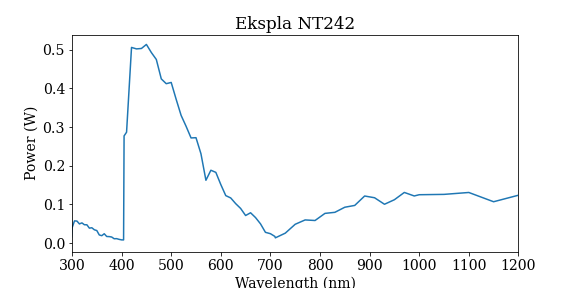
\includegraphics[width=\textwidth]{nt242_output.png}
    \caption{Expected Power output of NT242 Tunable Laser}
    \label{fig:laser_power}
\end{figure}


\subsection{White Light System}
plot of LEDs
Mechanical configuration
Optical model
Model output

\subsection{Projector}

\subsection{Monitoring systems}

We will want to measure precisely how much light from the laser is entering the CBP at a given wavelength so that we determine the exact fraction of that light that is captured by the LSST camera. In order to do that, we need to monitor the luminosity of the laser as it enters the integrating sphere as well as the spectral properties of the light. This data will be recorded for every measurement made with the CBP in such a way that it can be easily linked to the LSST camera image. 

\paragraph{\textbf{Photodiode}}

In order to monitor the exact amount of light injected into the CBP, we use a Hamamatsu S2281 Silicon Photodiode that has been precisely calibrated by NIST. 
This photodiode, which is mounted directly to the integrating sphere, has a sensitive area of 11 mm in diameter. It is read out by a Keithley 6517b electrometer. The electrometer can measure current, charge, resistance and voltage. Our uses of the CBP will likely use the charge and current modes. 

The electrometer can be read out as quickly as every 20 ms. There is a relationship between how long of an exposure you can take and the integration time. At the minimum integration time, you can take an exposure of $\sim$30 seconds. The data is saved in a fits file in the lfa with the elapsed time from the start of the exposure and the value measured. The range can be set to any value from X to Y. 

\paragraph{\textbf{Fiber Spectrograph}}

The spectral response of the injected light will be measured by a pair of fiber-fed spectrographs from Avantes SensLine, one for the blue wavelengths (range) and one for the red (range). These spectrographs will actually be housed in the central projection area in the center of the calibration screen. This is where light from the laser can be projected on the calibration screen. The fibers will be situated such that they will measure some fraction of reflected light within the projector box. When we want to measure the spectral response of the light, we will inject the fiber that runs to the calibration screen, take our measurement, and then send the laser light to the CBP. This assumes that the spectral response will not change from one output to another, which we will have to confirm.

The data from the spectrographs will be saved in a fits file in the lfa that will include the wavelength array and the counts measured by the spectrograph at that spacing.

\section{CBP}
The Rubin CBP was built by DFM Engineering. 
The design is essentially a Schmidt camera used in reverse. 
It includes a primary mirror of 33cm diameter, Schmidt Corrector and a 3-element Flat Field Corrector. 
It produces a beam with an aperture of 24.1 cm and a field of view of 4.1 degrees. 
The focal length of the CBP is 625mm, and with the LSST focal length at 10.1m, the magnification factor is 16. Therefore, a 100$\mu$m pinhole on the CBP would correspond to 1600 $\mu$m, or 160 pixels. 

\begin{table}[h!]
    \centering
    \begin{tabular}{|c|c|}
      \hline
       Aperture   & 24.1 cm \\
      \hline
      Focal Length   & 62.5 cm \\
      \hline
      Field of View & 4.1 degrees \\
      \hline
    \end{tabular}
    \caption{CBP Specifications}
    \label{tab:my_label}
\end{table}

The mount of the CBP allows movement in Azimuth and Elevation, with a swing diameter of 51.8". 
The locations are controlled by a Galil Digital Motor Controller (DMC) that is mounted on the azimuth housing. It controls the motors, reads the encoders, and interfaces to the control computer over ethernet. 
Additionally, the DMC controls the focus of the primary mirror and changes and rotates the masks. 
The azimuth and elevation stages are absolutely encoded with a Renishaw 26-bit on axis encoder. 


\begin{figure}[h]
    \centering
    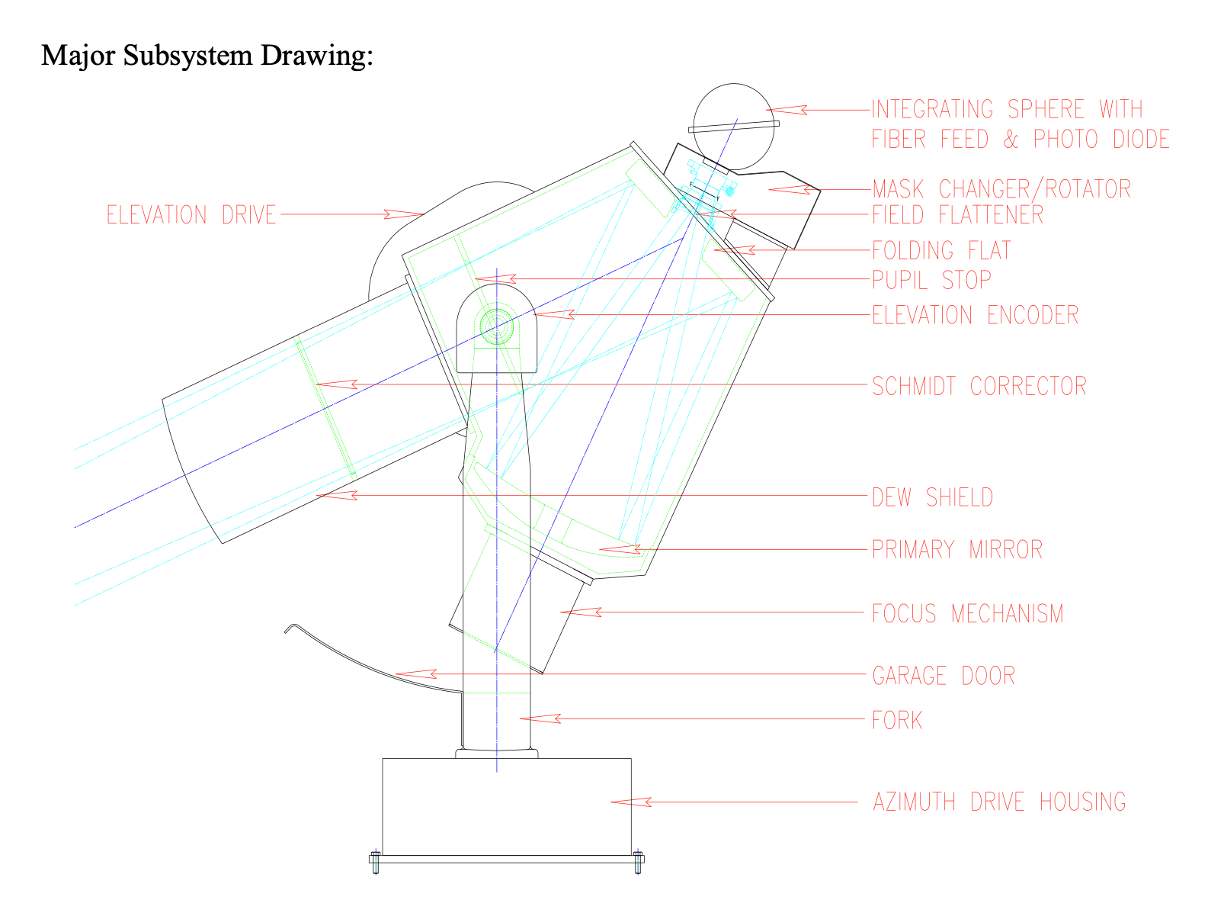
\includegraphics[width=\textwidth]{cbp_drawing.png}
    \caption{CBP Major subsystems}
    \label{fig:cbp_major_subsystems}
\end{figure}

At the focal plane sits the mask stage, which can hold 5 different masks. The masks can be rotated, driven by worm gears such that all masks are rotated on a common shaft by a single motor. The center mask stage is position encoded using a Renishaw absolute rotary encoder. The mask holder can hold masks with a diameter of 50 mm. Each mask will be laser etched into aluminium and are removable/interchangeable. 

The current Integrating Sphere installed on the CBP is a Labsphere 3P-GPS-060-SF. 
This integrating sphere has an interior diameter of 6 in. (152.4mm) and an exit port of 2.5 in. (63.5 mm), coated with spectraflect coating. 
In the exit port a photodiode will be mounted and it will be illuminated by an optical fiber.
The integrating sphere is held to the mask stage with standoffs. 
It sits $\sim 3$ in. from the focal plane/mask. 
Using \url{https://www.labsphere.com/wp-content/uploads/2021/09/Integrating-Sphere-Theory-and-Applications.pdf} as a guide to calculate the intensity of light exiting the integrating sphere by multiplying Ls by the flux incident on the integrating sphere.

\section{AuxTel/LATISS}

\section{Camera EOTest Data}

\section{On-Sky Data}
\subsection{Twilight Flats}
\subsection{Dense Dithered Star Fields}

\section{Plans Post-Year 1}
\subsection{Synethetic SED matched flats}
\subsection{Full CBP dataset}


 Make sure lsst-texmf/bin/generateAcronyms.py is in your path
\appendix
\section{Calibration Products List}

\begin{table}[h!]
    \begin{tabular}{|c|c|}
    Quantity & Product Description \\
    \hline \hline
    \textbf{Bias} & (combined) \\
    \hline
    \textbf{Dark} &  (combined) \\
    \hline
    \textbf{CTI} & what are these? \\  
    \hline
    \textbf{PTC} & Linearity + Gain \\
    \hline
    \textbf{C$_{i}$} & Crosstalk Matrix \\
    \hline
     & Defect masks \\
    \hline
    \textbf{BF} & Brighter-fatter kernels \\
    \hline
     & Fringe templates (zy) \\
    \hline
     & Lateral e-field templates \\
    \hline
    \textbf{QE$_{det}$} & Sensor QE \\ 
    \hline
    \textbf{R$_{mirror}$} & Mirror reflectivity (Silver x3) \\
    \hline
    \textbf{T$_{filter}$} & Filter transmission \\
    \hline
     & “White” light flats (ugrizy) \\ 
    \hline
    \textbf{T}(det, $\lambda$) & Transmission \\ 
    \hline
     & Dust flat (?) \\
    \hline
     & Twilight flats (ugrizy; combined) \\
    \hline
     & Sky flat (combined; ugrizy) \\
    \hline
     & Reference Flux Flat \\
    \hline
     & Dense dithered star field + lateral e-field (ugrizy) \\
    \hline
     & Survey observations \\
    \hline
    \end{tabular}
\end{table}


% Include all the relevant bib files.
% https://lsst-texmf.lsst.io/lsstdoc.html#bibliographies
\section{References} \label{sec:bib}
\renewcommand{\refname}{} % Suppress default Bibliography section
\bibliography{local,lsst,lsst-dm,refs_ads,refs,books}

\section{Acronyms} \label{sec:acronyms}
\addtocounter{table}{-1}
\begin{longtable}{p{0.145\textwidth}p{0.8\textwidth}}\hline
\textbf{Acronym} & \textbf{Description}  \\\hline

CBP & Collimated Beam Projector \\\hline
GPS & Global Positioning System \\\hline
ISR & Instrument Signal Removal \\\hline
LATISS & LSST Atmospheric Transmission Imager and Slitless Spectrograph \\\hline
LPM & LSST Project Management (Document Handle) \\\hline
LSE & LSST Systems Engineering (Document Handle) \\\hline
LSST & Legacy Survey of Space and Time (formerly Large Synoptic Survey Telescope) \\\hline
LTS & LSST Telescope and Site  (Document Handle) \\\hline
NIST & National Institute of Standards and Technology (USA) \\\hline
QE & quantum efficiency \\\hline
SE & System Engineering \\\hline
SED & Spectral Energy Distribution \\\hline
SF & Structure Function \\\hline
SRD & LSST Science Requirements; LPM-17 \\\hline
\end{longtable}

% If you want glossary uncomment below -- comment out the two lines above
%\printglossaries


\end{document}
